\documentclass[a4paper,12pt]{article}
\usepackage[utf8x]{inputenc}
\usepackage [T1]{fontenc}
\usepackage{datetime}
\usepackage{indentfirst}
\usepackage{subcaption}
\captionsetup{compatibility=false}
\usepackage[T2A]{fontenc}
\usepackage[hmargin={20mm,10mm},vmargin={20mm,15mm},bindingoffset=0mm]{geometry}
\usepackage[colorlinks=true, linkcolor=black, citecolor=blue, urlcolor=blue, unicode]{hyperref}


\usepackage{docstyle}



\begin{document}
\begin{titlepage}
	\centering
	{\scshape\large VILNIAUS UNIVERSITETAS \\
	MATEMATIKOS IR INFORMATIKOS FAKULTETAS \par}
	\vspace{6cm}
	{\huge\bfseries Kompiueterine rega. Teksto atpažinimas\par}
	{\LARGE Tiriamojo seminaro ataskaita\par}
	{\Large Matematinė informatika 3 kursas}
	\vspace{3cm}
	\vfill
	\flushright
	Autorius: \\ Ignas Jatulis\par
	\vspace{0.5cm}
	Vadovas: \\ Irus Grinis
	\vfill
	\centering
	{\the\year}
\end{titlepage}	
\tableofcontents

\newpage
\section*{Įvadas}
\addcontentsline{toc}{section}{Įvadas}

Šiais laikais žmonės vis daugiau veiksmų atlieka kompiuterio pagalba. 

Pavyzdžiui, jei seniau studentai sesijos metu, prieš egzaminus, konsektus rašydavo ranka, tai šiais laikais, vis daugiau studentų renkasi kompiuterį, jame esančias teksto rengikles, kurių pagalbą galima patogiai ir tvarkingai parengti konspektus. Tačiau sudarymi konspektus iš ranką rašytų sąsiuvinių, jie sugaištą nemažai laiko.  Tad kodėl nesukūrus programos ar mobiliosios programėlės, kurios pagalba užtektų nufotografuoti ar nuskenuoti tekstą, o kompiuteris jį pats atpažintų. 
Kodėl pasirinkta, kodel aktualu ir pns?

\newpage
\section{OpenCV biblioteka}
Nuotraukų apdorojimui buvo pasirinkta OpenCV biblioteka  (\cite{OpenCVabout}). OpenCV (Open Source Computer Vision Library) yra atvirojo kodo kompiuterinės regos biblioteka. Šią biblioteką galima naudoti tiek mokslo, tiek komercijos tikslais.\\
\indent Šioje kompiuterinės regos bibliotekoje yra realizuota daugiau kaip 2500 optimizuotų algoritmų kurie padeda apdirbti vaizdus. Taip pat ji pritaikyta programuoti su tokiomis kalbomis kaip C++, C, Python, JAVA ir yra suderinama su populiariausiomis operacinėmis sistemomis, tokiomis kaip Windows, Linux, Android ar Mac OS. Apie kiekvieną bibliotekoje esantį algoritmai ir jo panaudojimo pavyzdžius, galima rasti OpenCV dokumentacijoje  (\cite{OpenCVdoc}).

\newpage
\section{Nuotraukų apdorojimas teksto atpažinimui}


\newpage
\section{Pavyzdys}
Turime nuotrauką, kurioje yra nufotografuoti žodžiai parašyti ant popieriaus lapo.
\begin{center}
	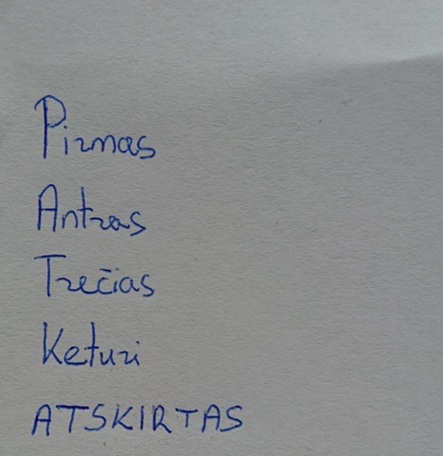
\includegraphics[scale=0.75]{img/1.png}\\
	\textbf{Pav. 1}: Nufotografuotas tekstas\\
\end{center}


\newpage
\section*{Išvados}
\addcontentsline{toc}{section}{Išvados}
Taigi, per šį semestrą buvo atliktas žodžių segmentavimas iš nuotraukų. Nuotraukoje esantys žodžiai išsaugomi kaip atskiri *.jpg formato paveiksliukai. Taip pat buvo bandoma, kuo optimaliau atlikti žodžių segmentaciją į raides. Jei žodžio raidės nėra sujungiamos, tai raides susegmentuodavo beveik 100\% tikslumu. Didžioji problema yra žodžio skaidymas, kai raidės yra sujungtos. Buvo bandoma spėti, jog vieta, per kurią reiktų skelti paveiksliuka ir jog tai raidžių susijungimo vieta, toje vietoje, kur linija jungianti raides įgyja mažiausią reikšmę, tai yra, ten, kur raides jungianti linija yra ploniausia. Atlikus testus paaiškėjo, jog toks segmentavimas efektingas tik apie 50 \% atvejų.\\
\indent Sekančiame semestre bus siekiama dar labiau patobulinti segmentavimo į raides algoritmą ir sukurti kelių sluoksnių neuroninį tinklą bei apmokyti kompiuterį atpažinti pateiktas raides.

\newpage
\renewcommand{\refname}{Literatūra}
\addcontentsline{toc}{section}{Literatūra}
\begin{thebibliography}{99}

\bibitem {OpenCVdoc}
OpenCV documentacija. 
\url{http://docs.opencv.org/}

\bibitem {OpenCVabout}
Apie OpenCV.
\url{http://opencv.org/about.html}
[Žiūrėta 2017 m. gegužės mėn.]

\bibitem {KavaliauskasFelinskas}
G.  Kavaliauskas, G. Felinskas. Dirbtinio intelekto atpažinimo metodų analizė ir taikymai ranka rašytam tekstui atpažinti. Jaunųjų mokslininkų darbai  (Nr. 4(37)), 2012, p. 205-211

\bibitem {Beigi}
H.S.M. Beigi.  An overview of handwriting recognition. Proceedings of the 1 st Annual Conference on Technological Advancements in Developing Countries, 1993, p. 30-46

\end{thebibliography}


\end{document}

